\documentclass[conference]{IEEEtran}
\IEEEoverridecommandlockouts
\usepackage{cite}
\usepackage{amsmath,amssymb,amsfonts}
\usepackage{graphicx}
\usepackage{booktabs}
\usepackage{multirow}
\usepackage{array}
\usepackage{xcolor}
\usepackage{tikz}
\usetikzlibrary{positioning,arrows.meta,shapes.geometric}
\usepackage{pgfplots}
\pgfplotsset{compat=1.17}
\usepackage[hidelinks]{hyperref}
\usepackage{url}
\def\BibTeX{{\rm B\kern-.05em{\sc i\kern-.025em b}\kern-.08em
    T\kern-.1667em\lower.7ex\hbox{\sc e}\kern-.125em X}}
\newcommand{\inr}{INR~}

\begin{document}

\title{UPI Guard: An Audited Pre-Debit Fraud-Risk Benchmark for UPI Payments with Learnability Testing, Out-of-Time Evaluation and INR Cost Analysis}

\author{\IEEEauthorblockN{Yogendra Pandey, Sahil Mangla, Kuldeep Khengar}
\IEEEauthorblockA{Goa Institute of Management --- Big Data Analytics\\
Student IDs: B2026109, B2026097, B2026082\\
Email: \{yogendra.pandey, sahil.mangla, kuldeep.devendrasinhkhengar\}2026b@gim.ac.in}}

\maketitle

\begin{abstract}
Real-time fraud screening for India's Unified Payments Interface (UPI) must decide, before a debit is authorised, whether to approve a payment or demand step-up verification. We build and evaluate such a pre-debit scorer on a public log of 250,000 UPI transactions from calendar year 2024 (480 labelled frauds, 0.192\% prevalence). Unlike our earlier drafts, every number reported here comes from one identified, seeded run, whose dataset hash, split counts and confusion counts are published. The pipeline (i)~removes the post-authorisation \texttt{transaction\_status} field and uses only 24 features available before debit, including past-only velocity counts; (ii)~separates training (Jan--Aug), calibration and threshold selection (Sep--Oct) and a single out-of-time test (Nov--Dec; 41,002 transactions, 77 frauds); (iii)~audits whether the label is learnable at all; and (iv)~converts scores into a net benefit in Indian rupees using the real transaction amounts. The audit finds no attribute associated with fraud after Benjamini--Hochberg correction (0 of 18 tests), and a label-permutation test gives $p=0.448$. Logistic regression, random forest, LightGBM, an MLP and a 1D-CNN reach test ROC-AUC between 0.495 and 0.565. The best, LightGBM at 0.565 (95\% CI [0.513, 0.621]), gives no reliable evidence of skill: it is not significant after Holm correction ($p=0.123$), lies below the minimum detectable AUC of 0.582, and contradicts its own training-window CV AUC of 0.492. At a review cost of \inr25, a flag pays for itself only above 1.66\% precision (8.7$\times$ the base rate), so the cost-optimal policy is to intervene on no transaction. A positive control with planted, simulated signal shows that the same pipeline recovers near-oracle discrimination (AUC 0.986 vs.\ oracle 0.993), so the null result reflects the data, not the method. A feature-order experiment shows that the 1D-CNN's convolutions add nothing. Its accuracy is insensitive to column order, it does not beat order-invariant models, and it trails them on PR-AUC. We conclude that this public dataset cannot support claims of production-grade UPI fraud detection, including the AUC of 0.999 in our earlier drafts, and we specify the data a real deployment would require.
\end{abstract}

\begin{IEEEkeywords}
UPI, payment fraud, pre-debit screening, data provenance, out-of-time validation, permutation test, calibration, cost-sensitive decision, positive control, tabular deep learning
\end{IEEEkeywords}

%=====================================================================
\section{Introduction}
%=====================================================================
UPI settles payments within seconds, so a fraudulent debit is rarely recoverable after the fact. The economically relevant intervention is therefore \emph{pre-debit}. At the moment the payer confirms a payment, the payer's bank or payment service provider (PSP) can approve the payment, or impose friction such as an additional authentication factor, a cooling-off delay or a manual review~\cite{rbi2024,npci2024}. A useful scorer must (a)~use only information that exists at that moment, (b)~output probabilities calibrated well enough to compare with a monetary cost, and (c)~be validated on a later time period than it was trained on, because fraud patterns drift~\cite{dalpozzolo2018}.

Our first-review manuscript reported AUC~0.9991 and equal precision and recall of 97.69\% for a 1D-CNN. The review identified three defects. The data provenance was unresolved. The sample sizes conflicted (31,250 versus 625 test rows). The metrics were internally inconsistent: at 0.192\% prevalence, recall 97.69\% and specificity 99.39\% imply a precision of only about 23.6\%, not 97.69\%. This paper replaces those results with a single traceable experiment. In doing so, it reaches a different and better-supported conclusion.

\textbf{Contributions.}
\begin{enumerate}
\item A \emph{feature-availability} protocol for pre-debit UPI screening. It drops authorisation outcomes, fits reference statistics on the training window only, and uses strictly backward-looking velocity counts, all enforced by unit tests (Sec.~\ref{sec:method}).
\item A \emph{learnability audit}: multiplicity-corrected association tests, a label-permutation test~\cite{ojala2010} and a power analysis. These should precede any reported fraud model (Sec.~\ref{sec:audit}).
\item A reconciled, \emph{out-of-time} comparison of six models. It reports bootstrap confidence intervals, exact TP/FP/FN/TN counts, calibration error, and a rupee-denominated net benefit with a break-even precision rule (Secs.~\ref{sec:models}--\ref{sec:business}).
\item A \emph{positive control} with planted signal that validates the pipeline's power. It also includes a controlled test of whether 1D convolutions over tabular columns carry any justified advantage (Sec.~\ref{sec:pc}).
\end{enumerate}

%=====================================================================
\section{Related Work}
%=====================================================================
\textbf{Fraud detection.} Bolton and Hand~\cite{bolton2002} frame fraud detection as supervised and unsupervised classification under extreme imbalance and label delay. Dal Pozzolo \emph{et al.}~\cite{dalpozzolo2018} show that realistic evaluation requires chronological splits and verification-latency-aware feedback. Whitrow \emph{et al.}~\cite{whitrow2009} and Bahnsen \emph{et al.}~\cite{bahnsen2016} show that the strongest card-fraud signals are customer-level aggregations, such as transaction velocity, deviation from the customer's own history, and periodic spending patterns. These need a persistent payer identifier.

\textbf{Synthetic financial data.} Public mobile-money and payment datasets are frequently simulated, as with PaySim~\cite{lopezrojas2016}, because real labelled transactions are confidential. Results on such data reflect the simulator's assumptions, so documenting provenance is essential~\cite{gebru2021,mitchell2019}.

\textbf{Evaluation under imbalance.} With prevalence near 0.2\%, ROC-AUC can look favourable while precision is very low. Precision--recall analysis is more informative~\cite{saito2015,davis2006}. Uncertainty in AUC can be quantified analytically~\cite{hanley1982,delong1988} or by bootstrap~\cite{efron1993}. Permutation tests establish whether a classifier beats chance~\cite{ojala2010}. Leakage from features unavailable at decision time is a common source of inflated results~\cite{kaufman2012}.

\textbf{Calibration and cost.} Cost-sensitive decisions need calibrated probabilities~\cite{elkan2001}. Platt scaling~\cite{platt1999} and isotonic regression~\cite{niculescu2005} are standard post-hoc methods. Isotonic regression overfits when positives are few~\cite{niculescu2005}. Resampling methods such as SMOTE~\cite{chawla2002} distort probabilities and must be corrected~\cite{dalpozzolo2015}.

\textbf{Deep learning on tables.} Large benchmarks find that tree ensembles such as LightGBM~\cite{ke2017} and random forests~\cite{breiman2001} still match or beat deep networks on typical tabular data~\cite{grinsztajn2022,shwartz2022}. Convolutions assume a meaningful local neighbourhood, which tabular column order does not provide.

%=====================================================================
\section{Data and Provenance}\label{sec:data}
%=====================================================================
\subsection{Source and integrity}
The study uses the file \texttt{upi\_transactions\_2024.csv} (SHA-256 prefix \texttt{8e46a45fd12c3e9e}; full hash in the repository manifest). It is a publicly redistributed transaction log with 250,000 rows and 17 columns, dated 2024-01-01 to 2024-12-30. It was \emph{not} released by NPCI, the RBI or any bank. It contains no payer, payee, account or device identifier, and no generating procedure is documented. Integrity checks found 0 missing values, 0 duplicate rows and 0 duplicate IDs. \texttt{hour\_of\_day}, \texttt{day\_of\_week} and \texttt{is\_weekend} are exactly consistent with \texttt{timestamp}. Amounts range from \inr10 to \inr42,099 (median \inr629). 480 rows are labelled fraud (0.192\%).

\textbf{Provenance statement.} Earlier drafts described this file both as ``empirical'' and as ``generated''. We now state only what can be verified: the file is public, and its origin is undocumented. Sec.~\ref{sec:audit} shows that its label behaves as if assigned independently of every recorded attribute, which is typical of a simulated dataset. We therefore treat it as a \emph{public benchmark of unknown, probably synthetic, origin}. No statement in this paper concerns real UPI fraud rates or losses.

\subsection{Feature availability at the pre-debit decision}
Table~\ref{tab:schema} classifies every column by whether it exists before authorisation. \texttt{transaction\_status} (SUCCESS/FAILED) is the outcome of authorisation. Using it would leak post-decision information~\cite{kaufman2012}, so it is excluded from all models. It is retained only in the audit.

\begin{table}[t]
\centering
\caption{Raw columns and their pre-debit availability}\label{tab:schema}
\footnotesize
\setlength{\tabcolsep}{3pt}
\begin{tabular}{@{}p{2.45cm}p{2.25cm}p{2.85cm}@{}}
\toprule
Column & Values & Pre-debit use \\
\midrule
transaction type & P2P, P2M, Bill, Recharge & Yes \\
merchant\_category & 10 categories & Yes \\
amount (INR) & 10--42,099 & Yes (log; train-fitted ratios) \\
sender/receiver age group & 5 brackets each & Yes (KYC) \\
sender\_state & 10 states & Yes \\
sender/receiver bank & 8 banks each & Yes (VPA lookup) \\
device\_type, network\_type & 3 / 4 levels & Yes \\
hour, weekday, weekend & from timestamp & Yes \\
timestamp & 2024 & Ordering, split, velocity \\
transaction\_status & SUCCESS/FAILED & \textbf{No}: post-authorisation \\
transaction id & unique & No: identifier \\
fraud\_flag & 0/1 & Target \\
\bottomrule
\end{tabular}
\end{table}

\subsection{Out-of-time split}
Rows are ordered by timestamp and split by calendar date (Table~\ref{tab:split}). The test window is scored exactly once, after all modelling choices are frozen.

\begin{table}[t]
\centering
\caption{Chronological split used in the reported run}\label{tab:split}
\footnotesize
\setlength{\tabcolsep}{3pt}
\begin{tabular}{@{}lcrrrr@{}}
\toprule
Split & Period & Rows & Frauds & Legit. & Rate (\%) \\
\midrule
Train & 2024-01-01\,--\,2024-08-31 & 167,149 & 316 & 166,833 & 0.189 \\
Validation & 2024-09-01\,--\,2024-10-31 & 41,849 & 87 & 41,762 & 0.208 \\
Test & 2024-11-01\,--\,2024-12-30 & 41,002 & 77 & 40,925 & 0.188 \\
\midrule
Total & & 250,000 & 480 & 249,520 & 0.192 \\
\bottomrule
\end{tabular}
\end{table}

%=====================================================================
\section{Methodology}\label{sec:method}
%=====================================================================
\begin{figure}[t]
\centering
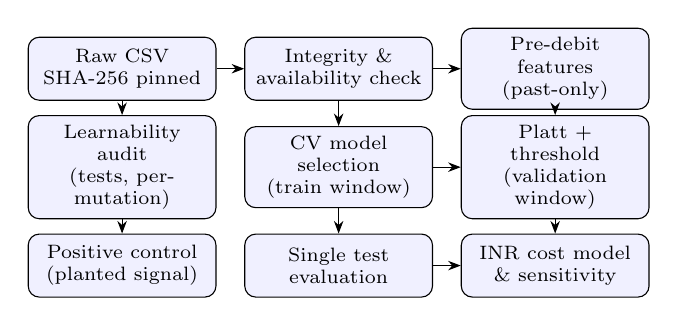
\begin{tikzpicture}[every node/.style={font=\scriptsize},
 box/.style={draw, rounded corners, fill=blue!6, align=center, minimum height=8mm, text width=2.15cm},
 >={Stealth[length=1.6mm]}]
\node[box] (a) at (0,0) {Raw CSV\\SHA-256 pinned};
\node[box] (b) at (2.75,0) {Integrity \&\\availability check};
\node[box] (c) at (5.5,0) {Pre-debit features\\(past-only)};
\node[box] (d) at (0,-1.25) {Learnability audit\\(tests, permutation)};
\node[box] (e) at (2.75,-1.25) {CV model selection\\(train window)};
\node[box] (f) at (5.5,-1.25) {Platt + threshold\\(validation window)};
\node[box] (i) at (0,-2.5) {Positive control\\(planted signal)};
\node[box] (g) at (2.75,-2.5) {Single test\\evaluation};
\node[box] (h) at (5.5,-2.5) {INR cost model\\\& sensitivity};
\draw[->] (a)--(b); \draw[->] (b)--(c); \draw[->] (c)--(f); \draw[->] (b)--(e); \draw[->] (e)--(f);
\draw[->] (a)--(d); \draw[->] (f)--(h); \draw[->] (e)--(g); \draw[->] (g)--(h); \draw[->] (d)--(i);
\end{tikzpicture}
\caption{UPI Guard pipeline. Each box corresponds to a module in the released code.}\label{fig:pipe}
\end{figure}

\subsection{Pre-debit feature engineering}
Let transaction $i$ occur at time $t_i$ with amount $a_i$ in merchant category $c_i$. We construct 24 inputs, grouped as follows.

\emph{Transaction:} $\log(1+a_i)$; the ratio $a_i/\tilde a_{c_i}$ to the training-window median of the category; the training-window percentile of $a_i$ within $c_i$; and an indicator $a_i > q_{0.95}(c_i)$. All reference statistics come from the training window only.

\emph{Temporal:} hour, $\sin(2\pi h/24)$, $\cos(2\pi h/24)$, a night flag (00:00--05:59), weekend, and weekday.

\emph{Party:} sender and receiver age groups, their absolute ordinal gap, sender state, sender and receiver banks, and a same-bank flag.

\emph{Device:} device and network type.

\emph{Velocity:} because no payer identifier exists, we use segment-level counts. The segment is $g_i = $ (sender bank, state, age group, device). The counts are
\begin{equation}
v_i^{(w)} = \big|\{\, j : g_j = g_i,\; t_i - w < t_j < t_i \,\}\big|,
\end{equation}
for $w\in\{1\,\text{h}, 24\,\text{h}\}$, plus a global 10-minute count. The strict inequality $t_j<t_i$ guarantees that only the past is used. A unit test confirms that appending future rows never changes a past row's features. No feature uses labels.

\subsection{Learnability audit}\label{sec:auditmethod}
For each attribute, we test independence from the label: Pearson $\chi^2$ for categorical attributes (with Cram\'er's $V$), and Mann--Whitney $U$ for numeric ones (with the univariate AUC $U/(n_1n_0)$). The 18 $p$-values are adjusted with Benjamini--Hochberg~\cite{bh1995}. For the joint question, we compute the 3-fold cross-validated AUC of an $L_2$ logistic regression on all pre-debit attributes. We compare it with the same statistic under 200 random permutations of the label, with $p = (1+\#\{\text{AUC}^{\pi}\ge \text{AUC}\})/(1+200)$~\cite{ojala2010}.

\textbf{Power.} Under $H_0$: AUC $=0.5$, the standard error of the empirical AUC is $\sqrt{(n_1+n_0+1)/(12 n_1 n_0)}$~\cite{hanley1982}. With $n_1=77$ test frauds, this is 0.0329. A one-sided 5\% test therefore requires AUC $>0.554$, and 80\% power requires a true AUC of at least \textbf{0.582}. Smaller real effects cannot be confirmed on one two-month test window.

\subsection{Models and selection}\label{sec:models}
We compare a prevalence baseline (constant prior), $L_2$ logistic regression (one-hot inputs, balanced class weights), a random forest~\cite{breiman2001} (300 trees, balanced bootstrap weights), LightGBM~\cite{ke2017}, an MLP (64--32 units, early stopping), and a 1D-CNN that re-implements our earlier architecture. The CNN has two \texttt{Conv1d} layers (32 and 64 filters, kernel~2) with batch normalisation and ReLU, dropout 0.25, a dense layer of 32 units, and a sigmoid output. It uses positive-class weight $\sqrt{n_0/n_1}$ over the 78 one-hot/scaled inputs. Small, pre-declared grids are searched by 5-fold stratified CV on the training window, using PR-AUC as the selection criterion. Selected settings: Logistic Regression: C=1.0; Random Forest: min\_samples\_leaf=100; LightGBM: num\_leaves=31, scale\_pos\_weight=1.0; MLP: alpha=0.01. We use class weights instead of SMOTE, because SMOTE distorts probability estimates~\cite{dalpozzolo2015}.

\subsection{Calibration and operating points}
Scores are recalibrated by Platt scaling~\cite{platt1999} on the validation window. We use Platt rather than isotonic regression because only 87 validation frauds are available~\cite{niculescu2005}. Expected calibration error (ECE) uses 10 equal-mass bins, because equal-width bins are almost empty at 0.2\% prevalence. Two operating points are fixed on validation and then applied unchanged to test: (a)~an \emph{alert budget} of 1\% of traffic, and (b)~the threshold that maximises validation net benefit (Sec.~\ref{sec:cost}). Option (b) may select ``flag nothing''.

\subsection{INR cost model}\label{sec:cost}
Let $r$ be the cost of one step-up or review (OTP, operations time, abandonment). Let $e\in[0,1]$ be the share of a flagged fraud that the intervention prevents. The net benefit of threshold $\theta$, relative to approving everything, is
\begin{equation}
B(\theta) = e \sum_{i} a_i\,\mathbb{1}[\hat p_i\ge\theta,\,y_i=1] \;-\; r \sum_i \mathbb{1}[\hat p_i\ge\theta].
\end{equation}
The amounts $a_i$ are the real recorded values, so the losses are in rupees. No currency conversion or invented per-incident loss is used. A flagged set is profitable only if its precision $P$ satisfies
\begin{equation}
P \;>\; P^{*} = \frac{r}{e\,\bar a_{\text{fraud}}}, \qquad \text{required lift} = P^{*}/\pi,
\end{equation}
where $\bar a_{\text{fraud}}=$\,\inr1,504 is the mean training-window fraud amount and $\pi$ is the prevalence. We take $r=$\,\inr25 and $e=1$ as the base case. The value $e=1$ is deliberately optimistic in the model's favour. We vary $r$ from \inr5 to \inr100. These are \emph{stated assumptions}, not measured bank costs.

\subsection{Positive control and CNN feature-order test}\label{sec:pcmethod}
To check that the pipeline \emph{can} detect fraud when it exists, we keep all real features and replace only the label with
\begin{equation}
y_i^{*}\sim\text{Bernoulli}\big(\sigma(\beta_0 + s\,z_i)\big),
\end{equation}
where $z_i$ is the standardised risk score of Table~\ref{tab:pcterms}. It includes a night$\times$high-amount interaction that a linear model cannot represent. $\beta_0$ is solved numerically so that the mean probability equals the real prevalence of 0.192\%. The strength $s$ ranges over $\{0,0.25,0.5,1,1.5,2\}$ with three label draws each. The case $s=0$ reproduces a label independent of the features. The \emph{oracle} AUC uses the true $\sigma(\beta_0+s z_i)$. These labels are simulated and are used only to validate the method. To test the convolutional premise, we retrain the CNN on five column orderings: the canonical order and four random permutations. We compare against order-invariant references (MLP, LightGBM) at $s=0$ (real labels) and at $s=1.5$.

\begin{table}[t]
\centering
\caption{Planted risk-score terms (positive control only)}\label{tab:pcterms}
\footnotesize
\begin{tabular}{@{}lr@{}}
\toprule
Term (binary indicator) & Weight \\
\midrule
Night hour (00:00-05:59) & 1.0 \\
Amount above category p95 (train-fitted) & 1.0 \\
Web device & 0.7 \\
Night x high amount (interaction) & 1.5 \\
Age gap $\geq$ 3 brackets & 0.6 \\
Segment velocity in top 5 \% (past 1 h) & 0.8 \\
P2P transfer above INR 5,000 & 0.6 \\
\bottomrule
\end{tabular}
\end{table}

%=====================================================================
\section{Results}
%=====================================================================
All results come from one run (seed 42, 2026-11-10, 45.0 minutes on 4 CPU cores). The full outputs are in the repository's \texttt{artifacts/} folder.

\subsection{Learnability audit}\label{sec:audit}
Table~\ref{tab:audit} lists all 18 association tests. The number with unadjusted $p<0.05$ is 1 (\texttt{sender\_age\_group}). Roughly 0.9 such results are expected by chance. After Benjamini--Hochberg correction, 0 remain significant (smallest adjusted $p=0.459$). The largest Cram\'er's $V$ is 0.0080. The fraud rate across the levels of every attribute stays within a narrow band around the overall 0.192\%. Jointly, the cross-validated AUC with the true labels is 0.5034. Under 200 label permutations, the null mean is 0.5005 (sd 0.0182, 95th percentile 0.5323), giving $p=0.448$ (Fig.~\ref{fig:perm}). The data therefore provide no evidence against the hypothesis that \texttt{fraud\_flag} is independent of all recorded attributes.

\begin{table*}[t]
\centering
\caption{Learnability audit on all 250,000 rows. Statistic: $\chi^2$ (dof) or univariate AUC (Mann--Whitney). Rate range: min--max fraud rate (\%) across levels.}\label{tab:audit}
\footnotesize
\begin{tabular}{@{}lccccc@{}}
\toprule
Attribute & Statistic & Rate range (\%) & Cram\'er's $V$ & $p$ & $p_{\text{BH}}$ \\
\midrule
\texttt{transaction\_type} & 2.32 (3) & 0.183--0.239 & 0.0030 & 0.508 & 0.991 \\
\texttt{merchant\_category} & 3.97 (9) & 0.148--0.214 & 0.0040 & 0.913 & 0.991 \\
\texttt{transaction\_status} & 0.23 (1) & 0.170--0.193 & 0.0010 & 0.634 & 0.991 \\
\texttt{sender\_age\_group} & 11.10 (4) & 0.125--0.229 & 0.0067 & 0.026 & 0.459 \\
\texttt{receiver\_age\_group} & 7.35 (4) & 0.143--0.230 & 0.0054 & 0.118 & 0.991 \\
\texttt{sender\_state} & 7.76 (9) & 0.158--0.232 & 0.0056 & 0.558 & 0.991 \\
\texttt{sender\_bank} & 9.20 (7) & 0.161--0.250 & 0.0061 & 0.238 & 0.991 \\
\texttt{receiver\_bank} & 1.82 (7) & 0.164--0.207 & 0.0027 & 0.969 & 0.991 \\
\texttt{device\_type} & 0.46 (2) & 0.181--0.206 & 0.0014 & 0.796 & 0.991 \\
\texttt{network\_type} & 2.73 (3) & 0.184--0.235 & 0.0033 & 0.435 & 0.991 \\
\texttt{day\_of\_week} & 3.65 (6) & 0.163--0.210 & 0.0038 & 0.725 & 0.991 \\
\texttt{hour\_of\_day} & 15.90 (23) & 0.057--0.304 & 0.0080 & 0.860 & 0.991 \\
\texttt{is\_weekend} & 0.31 (1) & 0.189--0.200 & 0.0011 & 0.576 & 0.991 \\
\texttt{amount\_inr} & AUC$_1$=0.500 & -- & -- & 0.991 & 0.991 \\
\texttt{amount\_to\_cat\_median} & AUC$_1$=0.512 & -- & -- & 0.364 & 0.991 \\
\texttt{seg\_count\_1h} & AUC$_1$=0.502 & -- & -- & 0.744 & 0.991 \\
\texttt{seg\_count\_24h} & AUC$_1$=0.502 & -- & -- & 0.895 & 0.991 \\
\texttt{global\_count\_10m} & AUC$_1$=0.494 & -- & -- & 0.645 & 0.991 \\
\bottomrule
\end{tabular}
\end{table*}

\begin{figure}[t]
\centering
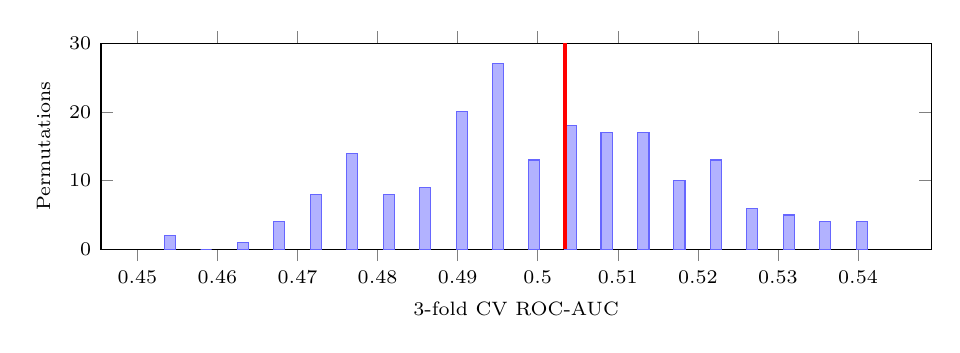
\begin{tikzpicture}
\begin{axis}[width=\columnwidth, height=4.2cm, ybar, bar width=4pt, xlabel={3-fold CV ROC-AUC}, ylabel={Permutations},
 ymin=0, ymax=30, tick label style={font=\scriptsize}, label style={font=\scriptsize},
 xticklabel style={/pgf/number format/fixed, /pgf/number format/precision=3}]
\addplot[fill=blue!30, draw=blue!60] coordinates {(0.4541,2.0000) (0.4586,0.0000) (0.4632,1.0000) (0.4677,4.0000) (0.4723,8.0000) (0.4768,14.0000) (0.4814,8.0000) (0.4859,9.0000) (0.4905,20.0000) (0.4950,27.0000) (0.4995,13.0000) (0.5041,18.0000) (0.5086,17.0000) (0.5132,17.0000) (0.5177,10.0000) (0.5223,13.0000) (0.5268,6.0000) (0.5314,5.0000) (0.5359,4.0000) (0.5405,4.0000)};
\draw[red, very thick] (axis cs:0.5034,0) -- (axis cs:0.5034,30);
\node[red, anchor=south west, font=\scriptsize] at (axis cs:0.5034,30) {};
\end{axis}
\end{tikzpicture}
\caption{Label-permutation null distribution of CV AUC (200 permutations). The red line is the true-label AUC (0.5034, $p=0.448$).}\label{fig:perm}
\end{figure}

\subsection{Out-of-time model comparison}
Table~\ref{tab:models} reports the single test evaluation. Training-window CV AUCs are all close to 0.5. On the Nov--Dec test window, the learned models reach ROC-AUC between 0.495 and 0.565. 4 of 5 bootstrap 95\% intervals (1,000 stratified resamples) contain 0.5. 1 unadjusted one-sided Mann--Whitney test(s) fall below 0.05, and 0 survive Holm correction for the five comparisons. The best point estimate is LightGBM (0.565). Its bootstrap interval [0.513, 0.621] has a lower bound only just above 0.5, but three observations argue against treating it as real skill. First, it is not significant once the five model comparisons are accounted for (Holm $p=0.123$). Second, the same configuration scored 0.492 in training-window CV and 0.511 on the validation window. Third, it lies below the minimum detectable AUC of 0.582. A single nominally significant result among five, which does not replicate across time windows, is what chance alone is expected to produce. PR-AUC values are at the prevalence level (1.88$\times10^{-3}$). Top-decile lift ranges from 0.65 to 1.30, compared with 1.0 for random ranking. Brier skill scores are essentially zero: no model predicts better than the constant base rate. Fig.~\ref{fig:roc} shows that all ROC curves follow the diagonal.

\begin{table*}[t]
\centering
\caption{Out-of-time test results (Nov--Dec 2024; 41,002 transactions, 77 frauds). CV AUC: 5-fold on training window (mean$\pm$sd). $p$: one-sided Mann--Whitney test of AUC$>$0.5, raw / Holm-adjusted. PR-AUC, Brier skill and ECE $\times10^{3}$; PR-AUC of random ranking $=$ 1.88.}\label{tab:models}
\footnotesize
\begin{tabular}{@{}lccccccc@{}}
\toprule
Model & CV AUC (train) & Test ROC-AUC [95\% CI] & $p$ raw / Holm & PR-AUC & Brier skill & ECE & Lift@10\% \\
\midrule
Prevalence baseline & -- & 0.500 [0.500, 0.500] & -- & 1.88 & -0.00 & 0.51 & 1.00 \\
Logistic Regression & 0.490$\pm$0.013 & 0.545 [0.479, 0.610] & 0.086 / 0.345 & 2.29 & -0.01 & 0.43 & 1.17 \\
Random Forest & 0.501$\pm$0.040 & 0.495 [0.436, 0.556] & 0.558 / 0.558 & 1.82 & -0.08 & 0.54 & 0.65 \\
LightGBM & 0.492$\pm$0.029 & 0.565 [0.513, 0.621] & 0.025 / 0.123 & 2.14 & -0.00 & 0.54 & 0.78 \\
MLP & 0.493$\pm$0.024 & 0.536 [0.472, 0.594] & 0.137 / 0.410 & 2.10 & -0.02 & 0.51 & 0.78 \\
1D-CNN & -- & 0.522 [0.454, 0.582] & 0.257 / 0.513 & 2.00 & -0.03 & 0.51 & 1.30 \\
\bottomrule
\end{tabular}
\end{table*}

\begin{figure}[t]
\centering
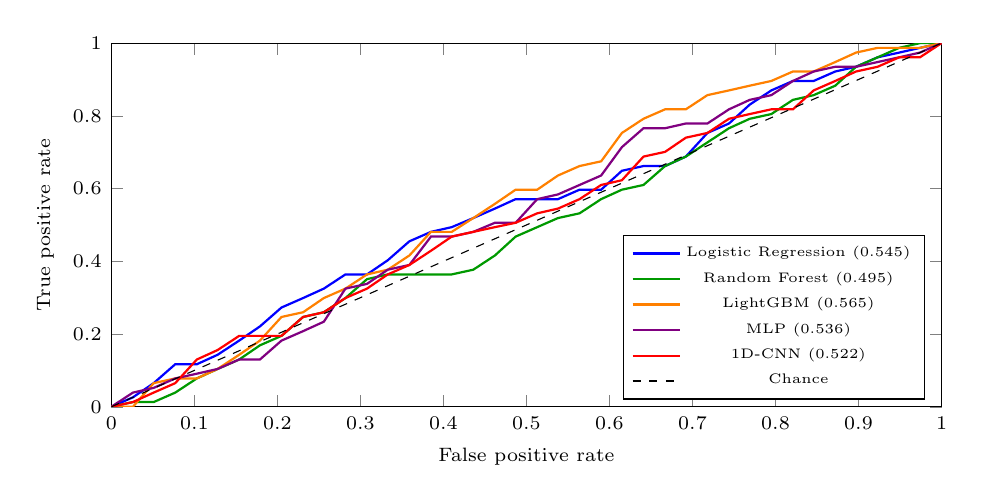
\begin{tikzpicture}
\begin{axis}[width=\columnwidth, height=6.2cm, xmin=0, xmax=1, ymin=0, ymax=1,
 xlabel={False positive rate}, ylabel={True positive rate},
 legend style={font=\tiny, at={(0.98,0.02)}, anchor=south east}, tick label style={font=\scriptsize}, label style={font=\scriptsize}]
\addplot[blue, thick] coordinates {(0.000,0.000) (0.026,0.026) (0.051,0.065) (0.077,0.117) (0.103,0.117) (0.128,0.143) (0.154,0.182) (0.179,0.221) (0.205,0.273) (0.231,0.299) (0.256,0.325) (0.282,0.364) (0.308,0.364) (0.333,0.403) (0.359,0.455) (0.385,0.481) (0.410,0.494) (0.436,0.519) (0.462,0.545) (0.487,0.571) (0.513,0.571) (0.538,0.571) (0.564,0.597) (0.590,0.597) (0.615,0.649) (0.641,0.662) (0.667,0.662) (0.692,0.688) (0.718,0.753) (0.744,0.779) (0.769,0.831) (0.795,0.870) (0.821,0.896) (0.846,0.896) (0.872,0.922) (0.897,0.935) (0.923,0.961) (0.949,0.974) (0.974,0.987) (1.000,1.000)};
\addlegendentry{Logistic Regression (0.545)}
\addplot[green!60!black, thick] coordinates {(0.000,0.000) (0.026,0.013) (0.051,0.013) (0.077,0.039) (0.103,0.078) (0.128,0.104) (0.154,0.130) (0.179,0.169) (0.205,0.195) (0.231,0.247) (0.256,0.260) (0.282,0.299) (0.308,0.351) (0.333,0.364) (0.359,0.364) (0.385,0.364) (0.410,0.364) (0.436,0.377) (0.462,0.416) (0.487,0.468) (0.513,0.494) (0.538,0.519) (0.564,0.532) (0.590,0.571) (0.615,0.597) (0.641,0.610) (0.667,0.662) (0.692,0.688) (0.718,0.727) (0.744,0.766) (0.769,0.792) (0.795,0.805) (0.821,0.844) (0.846,0.857) (0.872,0.883) (0.897,0.935) (0.923,0.961) (0.949,0.987) (0.974,1.000) (1.000,1.000)};
\addlegendentry{Random Forest (0.495)}
\addplot[orange, thick] coordinates {(0.000,0.000) (0.026,0.000) (0.051,0.065) (0.077,0.078) (0.103,0.078) (0.128,0.104) (0.154,0.143) (0.179,0.182) (0.205,0.247) (0.231,0.260) (0.256,0.299) (0.282,0.325) (0.308,0.364) (0.333,0.377) (0.359,0.416) (0.385,0.481) (0.410,0.481) (0.436,0.519) (0.462,0.558) (0.487,0.597) (0.513,0.597) (0.538,0.636) (0.564,0.662) (0.590,0.675) (0.615,0.753) (0.641,0.792) (0.667,0.818) (0.692,0.818) (0.718,0.857) (0.744,0.870) (0.769,0.883) (0.795,0.896) (0.821,0.922) (0.846,0.922) (0.872,0.948) (0.897,0.974) (0.923,0.987) (0.949,0.987) (0.974,0.987) (1.000,1.000)};
\addlegendentry{LightGBM (0.565)}
\addplot[violet, thick] coordinates {(0.000,0.000) (0.026,0.039) (0.051,0.052) (0.077,0.078) (0.103,0.091) (0.128,0.104) (0.154,0.130) (0.179,0.130) (0.205,0.182) (0.231,0.208) (0.256,0.234) (0.282,0.325) (0.308,0.338) (0.333,0.377) (0.359,0.390) (0.385,0.468) (0.410,0.468) (0.436,0.481) (0.462,0.506) (0.487,0.506) (0.513,0.571) (0.538,0.584) (0.564,0.610) (0.590,0.636) (0.615,0.714) (0.641,0.766) (0.667,0.766) (0.692,0.779) (0.718,0.779) (0.744,0.818) (0.769,0.844) (0.795,0.857) (0.821,0.896) (0.846,0.922) (0.872,0.935) (0.897,0.935) (0.923,0.948) (0.949,0.961) (0.974,0.974) (1.000,1.000)};
\addlegendentry{MLP (0.536)}
\addplot[red, thick] coordinates {(0.000,0.000) (0.026,0.013) (0.051,0.039) (0.077,0.065) (0.103,0.130) (0.128,0.156) (0.154,0.195) (0.179,0.195) (0.205,0.195) (0.231,0.247) (0.256,0.260) (0.282,0.299) (0.308,0.325) (0.333,0.364) (0.359,0.390) (0.385,0.429) (0.410,0.468) (0.436,0.481) (0.462,0.494) (0.487,0.506) (0.513,0.532) (0.538,0.545) (0.564,0.571) (0.590,0.610) (0.615,0.623) (0.641,0.688) (0.667,0.701) (0.692,0.740) (0.718,0.753) (0.744,0.792) (0.769,0.805) (0.795,0.818) (0.821,0.818) (0.846,0.870) (0.872,0.896) (0.897,0.922) (0.923,0.935) (0.949,0.961) (0.974,0.961) (1.000,1.000)};
\addlegendentry{1D-CNN (0.522)}
\addplot[black, dashed] coordinates {(0,0) (1,1)};
\addlegendentry{Chance}
\end{axis}
\end{tikzpicture}
\caption{Test-window ROC curves (Platt-calibrated scores). The AUC is shown in the legend.}\label{fig:roc}
\end{figure}

\subsection{Reconciled confusion counts}
Table~\ref{tab:conf} gives exact counts at the 1\% alert budget fixed on validation. All rows sum to the 41,002 test transactions and 77 frauds. Notably, LightGBM, the model with the highest test AUC, places 0 of the 77 frauds among its 412 alerts (TP=0, FP=412, FN=77, TN=40,513). Its small AUC gain therefore does not come from the high-risk tail, where an intervention would act. Across all models, at most one fraud falls in the top 1\%, against about 0.8 expected from random flagging. As an internal-consistency check, we recompute precision for every row from recall $R$, specificity $S$ and prevalence $\pi$ by Bayes' rule, $P=\frac{R\pi}{R\pi+(1-S)(1-\pi)}$. It matches the count-based value exactly. This is the identity that exposed the error in our first draft. Calibration matters for the class-weighted models. Logistic regression trained with balanced weights outputs raw scores near 0.5, giving ECE 475.2$\times10^{-3}$. Platt scaling on validation reduces this to 0.43$\times10^{-3}$. For LightGBM, ECE falls from 0.97 to 0.54 ($\times10^{-3}$). However, the calibrated probabilities are concentrated near the base rate, which is the calibrated answer when no signal exists.

\begin{table}[t]
\centering
\caption{Test confusion counts at a 1\% alert budget (threshold fixed on validation). Prec., Rec., Spec.\ in \%.}\label{tab:conf}
\footnotesize
\setlength{\tabcolsep}{3pt}
\begin{tabular}{@{}lrrrrrrrr@{}}
\toprule
Model & TP & FP & FN & TN & Prec. & Rec. & Spec. & Lift \\
\midrule
Logistic Regression & 1 & 384 & 76 & 40,541 & 0.26 & 1.30 & 99.06 & 1.38 \\
Random Forest & 0 & 376 & 77 & 40,549 & 0.00 & 0.00 & 99.08 & 0.00 \\
LightGBM & 0 & 412 & 77 & 40,513 & 0.00 & 0.00 & 98.99 & 0.00 \\
MLP & 1 & 385 & 76 & 40,540 & 0.26 & 1.30 & 99.06 & 1.38 \\
1D-CNN & 0 & 451 & 77 & 40,474 & 0.00 & 0.00 & 98.90 & 0.00 \\
\bottomrule
\end{tabular}
\end{table}

\subsection{Business impact in INR}\label{sec:business}
The test window contains 77 frauds totalling \inr111,882 (mean \inr1,453). With $r=$\,\inr25, the break-even precision is 1.66\%, i.e.\ 8.7$\times$ the base rate. No model reaches this lift. At the 1\% alert budget, LightGBM prevents \inr0 of fraud but incurs \inr10,300 of review cost, a net of \inr-10,300. When thresholds are chosen on validation to maximise net benefit, 2 of the 5 models select ``flag nothing'' (Table~\ref{tab:cost}). The others flag a few hundred transactions on the strength of validation noise, catch no fraud on test, and lose money. Fig.~\ref{fig:nb} shows that every model's net-benefit curve tracks the expectation for random flagging and decreases as more traffic is flagged. Table~\ref{tab:sens} varies the review cost. Even at \inr5 per review, the required lift exceeds what any model achieves, and the best realised test benefit across all costs and models is \inr0.

\begin{table}[t]
\centering
\caption{Test outcome of the validation-chosen cost-optimal policy ($r=$\,\inr25, $e=1$). $\theta=\infty$: flag nothing. Amounts in INR.}\label{tab:cost}
\footnotesize
\setlength{\tabcolsep}{2.5pt}
\begin{tabular}{@{}lrrrrrr@{}}
\toprule
Model & $\theta$ & Flags & Caught & Prevented & Review & Net \\
\midrule
Logistic Regression & $\infty$ & 0 & 0 & 0 & 0 & 0 \\
Random Forest & 0.00294 & 118 & 0 & 0 & 2,950 & -2,950 \\
LightGBM & 0.00227 & 598 & 0 & 0 & 14,950 & -14,950 \\
MLP & $\infty$ & 0 & 0 & 0 & 0 & 0 \\
1D-CNN & 0.00265 & 451 & 0 & 0 & 11,275 & -11,275 \\
\bottomrule
\end{tabular}
\end{table}

\begin{table}[t]
\centering
\caption{Sensitivity to review cost $r$ (INR). ``No-flag'': models whose validation-optimal policy flags nothing. Net: best test net benefit among models.}\label{tab:sens}
\footnotesize
\setlength{\tabcolsep}{3pt}
\begin{tabular}{@{}rrrcl r@{}}
\toprule
$r$ & $P^{*}$ (\%) & Lift req. & No-flag & Best model & Net \\
\midrule
5 & 0.33 & 1.7 & 1/5 & MLP & 0 \\
10 & 0.66 & 3.5 & 1/5 & MLP & 0 \\
25 & 1.66 & 8.7 & 2/5 & Logistic Regression & 0 \\
50 & 3.32 & 17.3 & 3/5 & Logistic Regression & 0 \\
100 & 6.65 & 34.6 & 3/5 & Logistic Regression & 0 \\
\bottomrule
\end{tabular}
\end{table}

\begin{figure}[t]
\centering
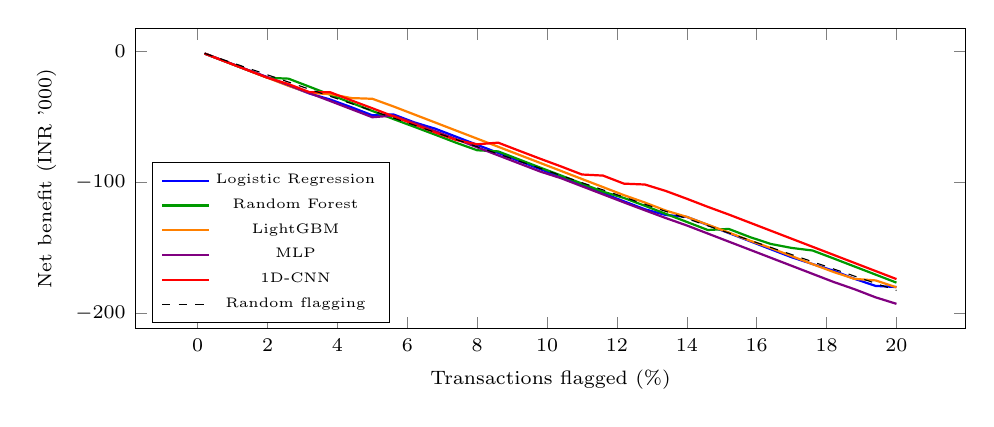
\begin{tikzpicture}
\begin{axis}[width=\columnwidth, height=5.4cm, xlabel={Transactions flagged (\%)}, ylabel={Net benefit (INR '000)},
 legend style={font=\tiny, at={(0.02,0.02)}, anchor=south west}, tick label style={font=\scriptsize}, label style={font=\scriptsize}]
\addplot[blue, thick] coordinates {(0.20,-2.05) (0.80,-8.05) (1.40,-14.20) (2.00,-20.19) (2.60,-26.34) (3.20,-32.49) (3.80,-37.13) (4.40,-42.96) (5.00,-49.11) (5.60,-48.41) (6.20,-54.49) (6.80,-59.31) (7.40,-65.46) (8.00,-71.61) (8.60,-77.76) (9.20,-83.91) (9.80,-90.06) (10.40,-96.21) (11.00,-102.36) (11.60,-108.51) (12.20,-114.66) (12.80,-120.72) (13.40,-125.10) (14.00,-126.54) (14.60,-132.69) (15.20,-138.84) (15.80,-144.99) (16.40,-151.14) (17.00,-157.29) (17.60,-162.49) (18.20,-167.56) (18.80,-173.71) (19.40,-179.13) (20.00,-180.01)};
\addlegendentry{Logistic Regression}
\addplot[green!60!black, thick] coordinates {(0.20,-2.05) (0.80,-8.20) (1.40,-14.35) (2.00,-20.50) (2.60,-21.17) (3.20,-27.32) (3.80,-33.47) (4.40,-39.62) (5.00,-45.77) (5.60,-51.92) (6.20,-57.88) (6.80,-63.89) (7.40,-70.04) (8.00,-75.74) (8.60,-76.62) (9.20,-82.77) (9.80,-88.92) (10.40,-94.99) (11.00,-101.14) (11.60,-107.29) (12.20,-112.12) (12.80,-118.07) (13.40,-124.22) (14.00,-130.37) (14.60,-136.52) (15.20,-135.71) (15.80,-141.86) (16.40,-147.15) (17.00,-150.19) (17.60,-152.16) (18.20,-158.20) (18.80,-164.35) (19.40,-170.50) (20.00,-176.65)};
\addlegendentry{Random Forest}
\addplot[orange, thick] coordinates {(0.20,-2.05) (0.80,-8.20) (1.40,-14.35) (2.00,-20.50) (2.60,-26.65) (3.20,-32.07) (3.80,-32.95) (4.40,-35.98) (5.00,-36.51) (5.60,-42.31) (6.20,-48.46) (6.80,-54.61) (7.40,-60.76) (8.00,-66.91) (8.60,-73.06) (9.20,-79.21) (9.80,-85.36) (10.40,-91.51) (11.00,-97.66) (11.60,-103.81) (12.20,-109.96) (12.80,-115.59) (13.40,-121.74) (14.00,-126.52) (14.60,-132.48) (15.20,-138.44) (15.80,-144.59) (16.40,-150.26) (17.00,-156.41) (17.60,-162.56) (18.20,-168.51) (18.80,-173.77) (19.40,-174.95) (20.00,-180.23)};
\addlegendentry{LightGBM}
\addplot[violet, thick] coordinates {(0.20,-2.05) (0.80,-8.11) (1.40,-14.26) (2.00,-20.09) (2.60,-26.05) (3.20,-32.20) (3.80,-38.27) (4.40,-44.42) (5.00,-50.58) (5.60,-49.32) (6.20,-55.03) (6.80,-61.18) (7.40,-67.33) (8.00,-73.48) (8.60,-79.63) (9.20,-85.78) (9.80,-91.93) (10.40,-97.05) (11.00,-103.20) (11.60,-109.35) (12.20,-115.50) (12.80,-121.51) (13.40,-127.45) (14.00,-133.06) (14.60,-139.22) (15.20,-145.37) (15.80,-151.51) (16.40,-157.66) (17.00,-163.81) (17.60,-169.97) (18.20,-176.12) (18.80,-181.67) (19.40,-187.82) (20.00,-192.80)};
\addlegendentry{MLP}
\addplot[red, thick] coordinates {(0.20,-2.05) (0.80,-8.20) (1.40,-14.35) (2.00,-20.50) (2.60,-25.28) (3.20,-31.43) (3.80,-31.59) (4.40,-37.74) (5.00,-43.73) (5.60,-49.88) (6.20,-56.03) (6.80,-62.18) (7.40,-67.96) (8.00,-71.20) (8.60,-69.95) (9.20,-76.10) (9.80,-82.17) (10.40,-88.08) (11.00,-94.23) (11.60,-95.04) (12.20,-101.19) (12.80,-101.86) (13.40,-106.79) (14.00,-112.72) (14.60,-118.87) (15.20,-124.73) (15.80,-130.88) (16.40,-137.03) (17.00,-143.18) (17.60,-149.33) (18.20,-155.48) (18.80,-161.63) (19.40,-167.78) (20.00,-173.93)};
\addlegendentry{1D-CNN}
\addplot[black, dashed] coordinates {(0.20,-1.83) (0.80,-7.31) (1.40,-12.78) (2.00,-18.26) (2.60,-23.74) (3.20,-29.22) (3.80,-34.70) (4.40,-40.18) (5.00,-45.66) (5.60,-51.14) (6.20,-56.62) (6.80,-62.10) (7.40,-67.57) (8.00,-73.05) (8.60,-78.53) (9.20,-84.01) (9.80,-89.49) (10.40,-94.97) (11.00,-100.45) (11.60,-105.93) (12.20,-111.41) (12.80,-116.89) (13.40,-122.36) (14.00,-127.84) (14.60,-133.32) (15.20,-138.80) (15.80,-144.28) (16.40,-149.76) (17.00,-155.24) (17.60,-160.72) (18.20,-166.20) (18.80,-171.68) (19.40,-177.15) (20.00,-182.63)};
\addlegendentry{Random flagging}
\end{axis}
\end{tikzpicture}
\caption{Test net benefit versus share of traffic flagged ($r=$\,\inr25, $e=1$). The dashed line is the expectation for random flagging.}\label{fig:nb}
\end{figure}

\subsection{Positive control}\label{sec:pc}
Fig.~\ref{fig:pc} and Table~\ref{tab:pc} show the planted-signal experiment. At $s=0$, all models score 0.508--0.523, reproducing the real-data result. As $s$ grows, the models track the oracle closely. At $s=0.5$, LightGBM reaches 0.626 against an oracle of 0.648. At $s=1.5$, the AUCs are 0.986 (LightGBM), 0.982 (random forest) and 0.982 (logistic regression), against an oracle of 0.993. The same INR cost model then yields a positive net benefit of \inr382,551. Even the weak signal at $s=0.5$ (oracle AUC 0.648) is already profitable (\inr42,769 for LightGBM). The break-even rule is therefore attainable whenever a real signal exists. Permutation importance on the planted setting ranks \texttt{seg\_count\_1h}, \texttt{hour\_of\_day}, \texttt{device\_type}, \texttt{age\_gap}, \texttt{high\_amount\_cat} highest. Each of these is an input to a planted term, so the explanation recovers the true drivers. Feature-group ablation (Table~\ref{tab:abl}) shows modest, consistent losses on planted labels (removing any group costs 0.006--0.017 AUC). The losses are small because the groups are partly redundant; for example, segment velocity encodes time of day. On the real labels, the ablation differences are within about one null standard error (0.0329) of each other, as expected for noise. The pipeline therefore has the power to find fraud signal of realistic size, and the absence of signal in the preceding subsections is a property of the dataset.

\begin{figure}[t]
\centering
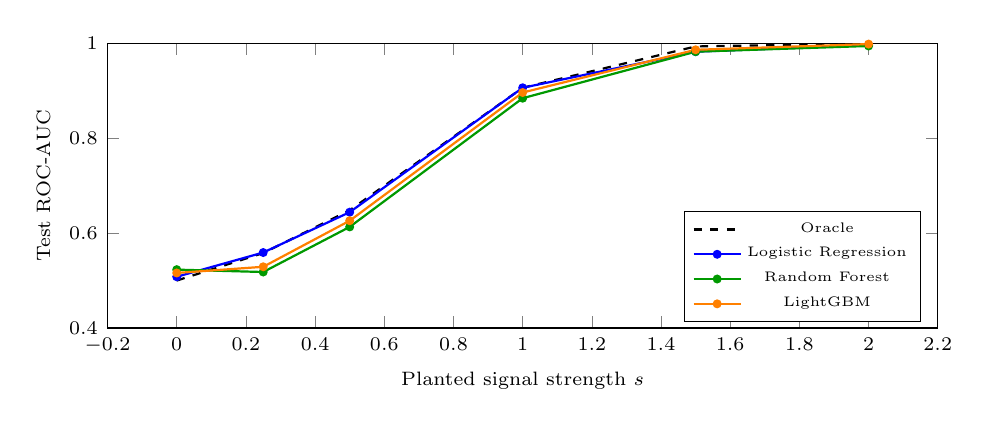
\begin{tikzpicture}
\begin{axis}[width=\columnwidth, height=5.2cm, xlabel={Planted signal strength $s$}, ylabel={Test ROC-AUC}, ymin=0.4, ymax=1.0,
 legend style={font=\tiny, at={(0.98,0.02)}, anchor=south east}, tick label style={font=\scriptsize}, label style={font=\scriptsize}]
\addplot[black, dashed, thick] coordinates {(0.000,0.500) (0.250,0.558) (0.500,0.648) (1.000,0.906) (1.500,0.993) (2.000,0.999)};
\addlegendentry{Oracle}
\addplot[blue, thick, mark=*, mark size=1.2pt] coordinates {(0.000,0.508) (0.250,0.559) (0.500,0.644) (1.000,0.906) (1.500,0.982) (2.000,0.996)};
\addlegendentry{Logistic Regression}
\addplot[green!60!black, thick, mark=*, mark size=1.2pt] coordinates {(0.000,0.523) (0.250,0.518) (0.500,0.613) (1.000,0.884) (1.500,0.982) (2.000,0.994)};
\addlegendentry{Random Forest}
\addplot[orange, thick, mark=*, mark size=1.2pt] coordinates {(0.000,0.516) (0.250,0.529) (0.500,0.626) (1.000,0.896) (1.500,0.986) (2.000,0.998)};
\addlegendentry{LightGBM}
\end{axis}
\end{tikzpicture}
\caption{Positive control on \emph{simulated} labels (mean of three draws). The models approach the oracle once a signal exists. At $s=0$, they reproduce the real-data result.}\label{fig:pc}
\end{figure}

\begin{table}[t]
\centering
\caption{Positive control: test ROC-AUC (mean$\pm$sd, 3 label draws) and LightGBM net benefit (INR, $r=25$). Simulated labels.}\label{tab:pc}
\footnotesize
\setlength{\tabcolsep}{2.5pt}
\begin{tabular}{@{}cccccr@{}}
\toprule
$s$ & Oracle & Logistic & Rand.\ forest & LightGBM & Net (INR) \\
\midrule
0.00 & 0.500 & 0.508$\pm$0.027 & 0.523$\pm$0.020 & 0.516$\pm$0.011 & 0 \\
0.25 & 0.558 & 0.559$\pm$0.015 & 0.518$\pm$0.041 & 0.529$\pm$0.040 & -1,559 \\
0.50 & 0.648 & 0.644$\pm$0.029 & 0.613$\pm$0.017 & 0.626$\pm$0.015 & 42,769 \\
1.00 & 0.906 & 0.906$\pm$0.024 & 0.884$\pm$0.023 & 0.896$\pm$0.019 & 250,392 \\
1.50 & 0.993 & 0.982$\pm$0.010 & 0.982$\pm$0.015 & 0.986$\pm$0.009 & 382,551 \\
2.00 & 0.999 & 0.996$\pm$0.004 & 0.994$\pm$0.004 & 0.998$\pm$0.001 & 428,144 \\
\bottomrule
\end{tabular}
\end{table}

\begin{table}[t]
\centering
\caption{Feature-group ablation (LightGBM test ROC-AUC)}\label{tab:abl}
\footnotesize
\begin{tabular}{@{}lcc@{}}
\toprule
Group removed & Real labels & Planted, $s$=1.5 \\
\midrule
None (all features) & 0.565 & 0.978 \\
Transaction & 0.519 & 0.961 \\
Temporal & 0.528 & 0.968 \\
Party/demographic & 0.561 & 0.971 \\
Device/network & 0.533 & 0.970 \\
Velocity (past-only) & 0.524 & 0.964 \\
\bottomrule
\end{tabular}
\end{table}

\subsection{Does the 1D-CNN's column order matter?}
Table~\ref{tab:cnn} shows the results. On real labels, the CNN is at chance under every ordering (0.487--0.534). On planted labels, the five orderings give almost identical ROC-AUC (0.977--0.981, sd 0.002), so column order is \emph{not} what the network exploits. After flattening, the dense layer sees every column, and the model behaves like an MLP with a small convolutional pre-processing step. It does not outperform the order-invariant references (MLP 0.975, LightGBM 0.978). It is clearly worse on PR-AUC, the metric that matters at 0.2\% prevalence (about 0.59--0.62 versus 0.68 and 0.70; Table~\ref{tab:cnn}). In the reported run it also took about 139\,s to train, against about 3\,s for LightGBM (run log). The premise of our earlier drafts, that local convolutions discover ``hierarchical feature correlations'' in tabular data, is therefore unsupported. This agrees with large tabular benchmarks~\cite{grinsztajn2022,shwartz2022}. We retain the CNN only as a comparison model.

\begin{table}[t]
\centering
\caption{1D-CNN feature-order sensitivity (test ROC-AUC; PR-AUC $\times10^3$)}\label{tab:cnn}
\footnotesize
\setlength{\tabcolsep}{3pt}
\begin{tabular}{@{}llcc@{}}
\toprule
Labels & Ordering / model & ROC-AUC & PR-AUC \\
\midrule
Real & canonical & 0.522 & 2.00 \\
Real & random \#1 & 0.534 & 2.08 \\
Real & random \#2 & 0.533 & 2.07 \\
Real & random \#3 & 0.520 & 2.04 \\
Real & random \#4 & 0.487 & 1.89 \\
Real & MLP (order-invariant reference) & 0.464 & 1.70 \\
Real & LightGBM (order-invariant reference) & 0.564 & 2.17 \\
Planted, $s$=1.5 & canonical & 0.977 & 606.73 \\
Planted, $s$=1.5 & random \#1 & 0.980 & 613.24 \\
Planted, $s$=1.5 & random \#2 & 0.981 & 584.78 \\
Planted, $s$=1.5 & random \#3 & 0.979 & 622.20 \\
Planted, $s$=1.5 & random \#4 & 0.978 & 589.23 \\
Planted, $s$=1.5 & MLP (order-invariant reference) & 0.975 & 676.03 \\
Planted, $s$=1.5 & LightGBM (order-invariant reference) & 0.978 & 700.70 \\
\bottomrule
\end{tabular}
\end{table}

\subsection{Latency}
Scoring one transaction end to end (feature construction, model and calibration) on one CPU took a median of 16.8~ms for logistic regression and 17.1~ms for LightGBM (95th percentile 25.7~ms). The random forest took 97.8~ms, dominated by parallel-dispatch overhead. Most of the single-row time is spent constructing the pandas feature frame; a vectorised or compiled feature path would reduce it. These times exclude the network and feature-store lookups that a production authorisation path would add.

%=====================================================================
\section{Discussion}
%=====================================================================
\subsection{Reconciliation with earlier versions}
Table~\ref{tab:recon} maps each earlier claim to its status. The earlier figures cannot be regenerated from this file under any leakage-free protocol we tested. The audit indicates why: the label carries no detectable information about the attributes. Any near-perfect score on this file must therefore come from leakage, a different dataset or a reporting error. We withdraw those claims.

\begin{table}[t]
\centering
\caption{Earlier claims versus this run}\label{tab:recon}
\footnotesize
\begin{tabular}{@{}p{3.1cm}p{4.6cm}@{}}
\toprule
V1/V2 claim & Status in this run \\
\midrule
AUC 0.9991 (1D-CNN) & Not reproducible. Test AUC 0.522; best model 0.565. \\
Precision = recall = 97.69\% & Internally inconsistent (implied precision $\approx$23.6\%). At a 1\% alert budget, the best model catches 1 of 77 frauds (precision $\le$0.26\%). \\
Test set 31,250 \emph{and} 625 rows & One test window: 41,002 rows, 77 frauds (Nov--Dec). \\
``Empirical'' and ``generated'' data & Public, undocumented origin; label independent of attributes. \\
\$6.35M savings at \$50K/fraud & Replaced by INR model on real amounts; optimal policy saves \inr0. \\
Telemetry adds +0.15\% AUC & On real labels, group ablation differences lie within noise (null SE 0.0329; Table~\ref{tab:abl}). \\
Latency $<$12\,ms & Measured end to end in Python: 17.1\,ms (LightGBM, median). \\
\bottomrule
\end{tabular}
\end{table}

\subsection{What a deployable UPI scorer would need}
The positive control shows what is missing in the data, not in the method. Card-fraud practice~\cite{whitrow2009,bahnsen2016} indicates that the predictive signals are entity-level. Examples are a payer's velocity and amount deviation relative to their own history, payee novelty (first payment to this VPA), device and SIM changes, collect-request patterns and beneficiary mule scores. Every one of these needs a persistent pseudonymous payer, payee and device identifier, which the public file lacks. A real study would also need the label confirmation delay, to avoid using unconfirmed recent labels~\cite{dalpozzolo2018}. It would need several months of out-of-time tests; Sec.~\ref{sec:auditmethod} shows that 77 frauds cannot confirm an AUC below 0.582. Finally, it would need measured intervention costs and abandonment rates in place of our assumed \inr25.

\subsection{Threats to validity}
\emph{Construct:} the meaning of \texttt{fraud\_flag} is undocumented. \emph{Internal:} hyper-parameter grids were small. With no signal, larger grids would only increase the risk of selection noise, and the positive control shows that the chosen settings are adequate when signal exists. \emph{External:} the conclusions apply to this file; they do not show that UPI fraud is unpredictable. \emph{Ethical:} age-based features could produce disparate step-up rates and must be monitored by group if used on real data~\cite{mitchell2019}.

%=====================================================================
\section{Reproducibility}
%=====================================================================
Code, the dataset hash, all artifacts and a Streamlit application are in the project repository: \url{https://github.com/yogendra9476/UPI-Guard-Fraud-Detection}. The following commands reproduce every table and figure.
\begin{enumerate}
\item \texttt{pip install -r requirements.txt} (plus \texttt{torch} for the CNN). The reported run used Python 3.13.18, scikit-learn 1.9.1, LightGBM 4.7.0, pandas 3.0.5, NumPy 2.5.3 and PyTorch 2.15.0+cu132.
\item \texttt{python run\_pipeline.py}: one seeded run (seed 42), which writes \texttt{artifacts/manifest.json} with the SHA-256 of the data (\texttt{8e46a45fd12c3e9e\ldots}), the split counts and all metrics.
\item \texttt{python build\_report.py}: inserts every number in this paper from the artifacts into the \LaTeX{} source, so the text cannot drift from the run.
\item \texttt{pytest -q}: twelve tests covering schema, chronological disjointness, absence of post-authorisation inputs, past-only velocity, train-only statistics, the precision identity and the cost model.
\item \texttt{streamlit run app.py}: an eight-page application for data exploration, the audit, results, the positive control, interactive INR cost analysis, live single and batch pre-debit scoring, and the reproducibility record.
\end{enumerate}
A data card and a model card document scope, intended use and limitations~\cite{gebru2021,mitchell2019}.

%=====================================================================
\section{Conclusion}
%=====================================================================
We rebuilt our UPI fraud study as a single traceable experiment designed around the pre-debit decision. On the supplied public dataset, a learnability audit, five learned models and an INR cost model agree. The fraud label is not reliably predictable from any pre-debit attribute. The best out-of-time AUC is 0.565 [0.513, 0.621], which is not significant after multiplicity correction and is not replicated across time windows, and the cost-optimal policy is not to intervene. A positive control shows that the same pipeline recovers near-oracle performance and positive rupee benefit when a signal exists. The 1D-CNN's convolutions provide no advantage over order-invariant models. The contribution is therefore methodological. Pre-debit feature discipline, learnability testing, power analysis, reconciled counts and break-even precision should accompany any reported fraud model, especially one trained on public data of uncertain provenance. Future work will apply the released pipeline to a labelled dataset with persistent entity identifiers and confirmed label dates.

\section*{Acknowledgment}
We thank the course instructors and the first-review panel, whose detailed feedback motivated this reconstruction. We used scikit-learn~\cite{pedregosa2011}, LightGBM, PyTorch, pandas, Streamlit and pgfplots. Generative AI tools were used to assist with code refactoring and language editing. All experimental results were produced by the released code and checked by the authors.

\begin{thebibliography}{99}\footnotesize
\bibitem{rbi2024} Reserve Bank of India, ``Annual Report 2023--24,'' Mumbai, May 2024.
\bibitem{npci2024} National Payments Corporation of India, ``UPI product statistics,'' 2024. [Online]. Available: \url{https://www.npci.org.in/what-we-do/upi/product-statistics}
\bibitem{bolton2002} R.~J. Bolton and D.~J. Hand, ``Statistical fraud detection: A review,'' \emph{Statistical Science}, vol.~17, no.~3, pp.~235--255, 2002.
\bibitem{dalpozzolo2018} A.~Dal~Pozzolo, G.~Boracchi, O.~Caelen, C.~Alippi, and G.~Bontempi, ``Credit card fraud detection: A realistic modeling and a novel learning strategy,'' \emph{IEEE Trans. Neural Netw. Learn. Syst.}, vol.~29, no.~8, pp.~3784--3797, 2018.
\bibitem{dalpozzolo2015} A.~Dal~Pozzolo, O.~Caelen, R.~A. Johnson, and G.~Bontempi, ``Calibrating probability with undersampling for unbalanced classification,'' in \emph{Proc. IEEE Symp. Comput. Intell. Data Mining (CIDM)}, 2015, pp.~159--166.
\bibitem{whitrow2009} C.~Whitrow, D.~J. Hand, P.~Juszczak, D.~Weston, and N.~M. Adams, ``Transaction aggregation as a strategy for credit card fraud detection,'' \emph{Data Mining Knowl. Discov.}, vol.~18, no.~1, pp.~30--55, 2009.
\bibitem{bahnsen2016} A.~Correa~Bahnsen, D.~Aouada, A.~Stojanovic, and B.~Ottersten, ``Feature engineering strategies for credit card fraud detection,'' \emph{Expert Syst. Appl.}, vol.~51, pp.~134--142, 2016.
\bibitem{lopezrojas2016} E.~A. Lopez-Rojas, A.~Elmir, and S.~Axelsson, ``PaySim: A financial mobile money simulator for fraud detection,'' in \emph{Proc. 28th European Modeling and Simulation Symp.}, 2016, pp.~249--255.
\bibitem{gebru2021} T.~Gebru \emph{et al.}, ``Datasheets for datasets,'' \emph{Commun. ACM}, vol.~64, no.~12, pp.~86--92, 2021.
\bibitem{mitchell2019} M.~Mitchell \emph{et al.}, ``Model cards for model reporting,'' in \emph{Proc. ACM FAT*}, 2019, pp.~220--229.
\bibitem{saito2015} T.~Saito and M.~Rehmsmeier, ``The precision-recall plot is more informative than the ROC plot when evaluating binary classifiers on imbalanced datasets,'' \emph{PLOS ONE}, vol.~10, no.~3, e0118432, 2015.
\bibitem{davis2006} J.~Davis and M.~Goadrich, ``The relationship between precision-recall and ROC curves,'' in \emph{Proc. 23rd ICML}, 2006, pp.~233--240.
\bibitem{hanley1982} J.~A. Hanley and B.~J. McNeil, ``The meaning and use of the area under a receiver operating characteristic (ROC) curve,'' \emph{Radiology}, vol.~143, no.~1, pp.~29--36, 1982.
\bibitem{delong1988} E.~R. DeLong, D.~M. DeLong, and D.~L. Clarke-Pearson, ``Comparing the areas under two or more correlated receiver operating characteristic curves: A nonparametric approach,'' \emph{Biometrics}, vol.~44, no.~3, pp.~837--845, 1988.
\bibitem{efron1993} B.~Efron and R.~J. Tibshirani, \emph{An Introduction to the Bootstrap}. New York: Chapman \& Hall, 1993.
\bibitem{ojala2010} M.~Ojala and G.~C. Garriga, ``Permutation tests for studying classifier performance,'' \emph{J. Mach. Learn. Res.}, vol.~11, pp.~1833--1863, 2010.
\bibitem{bh1995} Y.~Benjamini and Y.~Hochberg, ``Controlling the false discovery rate: A practical and powerful approach to multiple testing,'' \emph{J. R. Stat. Soc. B}, vol.~57, no.~1, pp.~289--300, 1995.
\bibitem{kaufman2012} S.~Kaufman, S.~Rosset, C.~Perlich, and O.~Stitelman, ``Leakage in data mining: Formulation, detection, and avoidance,'' \emph{ACM Trans. Knowl. Discov. Data}, vol.~6, no.~4, pp.~1--21, 2012.
\bibitem{elkan2001} C.~Elkan, ``The foundations of cost-sensitive learning,'' in \emph{Proc. 17th IJCAI}, 2001, pp.~973--978.
\bibitem{platt1999} J.~Platt, ``Probabilistic outputs for support vector machines and comparisons to regularized likelihood methods,'' in \emph{Advances in Large Margin Classifiers}, MIT Press, 1999, pp.~61--74.
\bibitem{niculescu2005} A.~Niculescu-Mizil and R.~Caruana, ``Predicting good probabilities with supervised learning,'' in \emph{Proc. 22nd ICML}, 2005, pp.~625--632.
\bibitem{chawla2002} N.~V. Chawla, K.~W. Bowyer, L.~O. Hall, and W.~P. Kegelmeyer, ``SMOTE: Synthetic minority over-sampling technique,'' \emph{J. Artif. Intell. Res.}, vol.~16, pp.~321--357, 2002.
\bibitem{ke2017} G.~Ke \emph{et al.}, ``LightGBM: A highly efficient gradient boosting decision tree,'' in \emph{Advances in NeurIPS}, vol.~30, 2017.
\bibitem{breiman2001} L.~Breiman, ``Random forests,'' \emph{Machine Learning}, vol.~45, no.~1, pp.~5--32, 2001.
\bibitem{grinsztajn2022} L.~Grinsztajn, E.~Oyallon, and G.~Varoquaux, ``Why do tree-based models still outperform deep learning on typical tabular data?'' in \emph{Advances in NeurIPS (Datasets and Benchmarks)}, vol.~35, 2022.
\bibitem{shwartz2022} R.~Shwartz-Ziv and A.~Armon, ``Tabular data: Deep learning is not all you need,'' \emph{Information Fusion}, vol.~81, pp.~84--90, 2022.
\bibitem{pedregosa2011} F.~Pedregosa \emph{et al.}, ``Scikit-learn: Machine learning in Python,'' \emph{J. Mach. Learn. Res.}, vol.~12, pp.~2825--2830, 2011.
\end{thebibliography}

\end{document}
